\section{Wstęp}

\qquad Elektrokardiogram jest jednym z najefektywniejszych narzędzi diagnostycznych do wykrywania chorób serca. ECG dostarcza prawie wszystkich informacji o aktywności elektrycznej serca. Typowy sygnał ECG składa się z załamka P, zespołu QRS oraz załamków T i U. Spośród wszystkich tych elementów sygału elektrokardiograficznego najbardziej charakterystycznym i zarazem najbardziej znaczącym jest zespół QRS. Na podstawie jego kształtu można zdiagnozować różne dysfunkcje serca, dlatego jego automatyczna klasyfikacja jest ważnym zagadnieniem.

\qquad Zespół QRS opisuje pobudzenie mięśni serca i składa się z jednego lub kilku załamków określanych jako Q, R i S.
\begin{itemize}
	\item Załamek R – każdy załamek dodatni w obrębie zespołu QRS
	\item Załamek Q – pierwszy ujemny załamek widoczny przed załamkiem R
	\item Załamek S – pierwszy ujemny załamek widoczny po załamku R
\end{itemize}

Przykładowy (wyidealizowany) zespół QRS widoczny jest na rys. \ref{fig:QRSComplex}, przedstawiającym schematyczny fragment zapisu elektrokardiograficznego.


\begin{figure}[h]
	\centering
	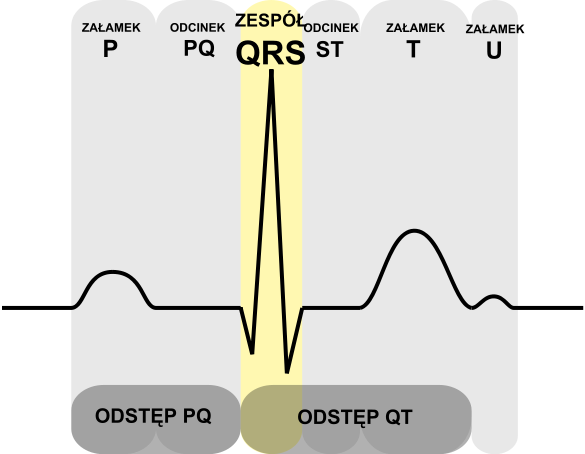
\includegraphics[width=0.8\textwidth]{Grafika/ZespolQRS}
	\caption{Wyidealizowany schemat zapisu EKG z zaznaczonym zespołem QRS. Źródło  \cite{QRSComplexWiki}}
	\label{fig:QRSComplex}
\end{figure}

\qquad Celem opisywanego modułu jest wyliczenie liczby klas zespołów QRS, określenie reprezentantów każdej z nich oraz oznaczenie klas zespołów QRS na wykresie ECG. Wyodrębnienie klas QRS występujących w sygnale ECG pozwala na określenie prawidłowości rytmu pracy serca. Z reguły nieregularności mają charakter przejściowy, dlatego ich poprawne wyznaczenie wymaga przeprowadzenia 24-godzinnego badania pracy serca, czyli testu Holtera \cite{RaportKoncowy}.

\qquad W literaturze można spotkać się z różnymi podejściami do klasyfikacji zespołów QRS. W \cite{SVMBasedArrhythmiaClassification} autorzy zaproponowali algorytm polegający na wykorzystaniu liniowej analizy dyskryminacyjnej (LDA) w celu zredukowania wymiaru przestrzeni cech. Do klasyfikacji zastosowano maszynę wektorów nośnych (SVM). Ponadto w pracy tej podjęto próbę klasyfiacji przy pomocy MLP (ang. Multilayer Perceptrons) oraz klasyfikatora FIS (ang. Fuzzy Inference System). Najlepsze rezultaty autorzy otrzymali wykorzystując SVM. Podobne podejście zastosowano w \cite{Abhishek}, gdzie dodatkowo w celu ograniczenia zakłóceń oraz ekstrakcji cech wykorzystano transformację falkową. 
W \cite{Laguna} autorzy stworzyli adaptacyjny algorytm, działający w czasie rzeczywistym, klasyfikujący zespoły QRS. Zaproponowane rozwiązanie bazuje na modelu funkcji Hermite'a. 
W innej pracy autorzy wyekstrahowali cztery konkretne cechy z sygnału ECG, aby następnie wykorzystać odległość Mahalanobisa jako kryterium klasyfikacji \cite{Moreas}.

\qquad Rozwiązanie przyjęte w niniejszej pracy opiera się o ekstrakcję cech z sygnału ECG, klasteryzacji otrzymanych wektorów przy pomocy algorytmu g-means oraz klasyfikacji z wykorzystaniem maszyny wektorów nośnych. Podejście takie podyktowane jest ... / wynika z ... ? TODO: NAPISAC JAKOS ZE WYKORZYSTUJEMY TO CO NAPISALI ROK TEMU


DO ZROBIENIA WE WSTĘPIE:
\begin{enumerate}
	\item cel (jest) i założenia projektu
	\item badania literaturowe - istniejące rozwiązania (vide linki, które wysłałem) 
	\item skróconą koncepcję rozwiązania (ekstrakcja - klasteryzacja - klasyfikacja)
\end{enumerate}